\documentclass[12pt]{article}

\usepackage[utf8]{inputenc}
\usepackage[margin=1in]{geometry}
\usepackage[titletoc,title]{appendix}
\usepackage[section]{placeins}  % allows us to stop floaters
\usepackage{longtable}  % for bringing in our data tables to the appendix
\usepackage{amsmath,amsfonts,amssymb,mathtools}
\usepackage{graphicx,float}
\usepackage{makecell}
\usepackage{caption}
\usepackage{csvsimple,booktabs} % load csv data into table
\usepackage{filecontents} % read csv data contents
\usepackage{indentfirst} % set first paragraph of each section to be indented
\usepackage[backend=biber,style=authoryear]{biblatex} % style our references

\addbibresource{references.bib} % load resources from bib file
\setlength{\parindent}{1.5em} % set indent length for each paragraph
\graphicspath{ {../figures/} }

\newcommand*\mean[1]{\overline{#1}}

\title{EOSC 453 Assignment 2\\
\large Volcanic Eruptions and Climate Change}
\author{
    E. Giroud-Proeschel - 123456789 \\
    P. Matlashewski - 45701109\\
    M. Ormerod - 16265167
}

\begin{document}

\maketitle
\newpage
\tableofcontents
\newpage

% Introduction and Overview
\section{Introduction}
Anthropogenic global warming is an identifier of climate change and a defining 
issue of our time. It is thought to be the main trigger of intensified, more frequent
extreme weather events, sea-level rise with the potential
to displace millions, and loss of large freshwater reservoirs.
The question of why, and how, climate change operates, and what we can do to mitigate 
its effects during our lifetime, is an arduously nonlinear problem that climate scientists
still battle with, both in the laboratory and in politics. Within this contention, we focus on
how large local out-gassing events of volatils such as sulfur dioxide during volcanic eruptions
have historically affected the Earth's climate. Here we chose to investigate
the impact of volcanic perturbations on a simple radiative
energy balance model. Throughout this paper we will only consider the effect of aerosols,
and more specifically, SO2. This model is inspired by the
work of Russian climatologist Mikhail I. Budyko, who discovered the ice-albedo
feedback mechanism underlying climate change through his pioneering of studies
on global climate using physical models of equilibrium (eq of what???) (\cite{budyko_albedo}).
We proceed as follows:

\begin{enumerate}
    \item Build a graphical algorithm solving the radiative energy balance equations in a zonally-averaged Earth model,
    based on figure 1
    \item Compute the present, steady-state energy balance of the Earth to investigate the effect of
    intra-zonal transfer by:
        \item setting all transfer coefficients kij to zero
        \item using the provided values of kij and comparing heat transfer magnitude and rates from our previous step
    \item from \cite(Robock 2000) from the 1982 El Chichón and Pinatubo eruption introduce a $\phi(t)$ function representing the spatially
    and temporally reducing effects of aerosol outgassing on the incoming radiation
    \item Consider a nonlinear effect of temperature on albedo.
    \item Using this new albedo parameterization as a proxy for the "ice-albedo" feedback, we look for solutions favourable to Snowball Earth
conditions.
    \item We then implement a Poisson sampling of eruptions to investigate a volcanic solution to Snowball Earth  
\end{enumerate}

% Anthropogenic global warming is an identifier of climate change and a defining 
% issue of our time. It is thought to be the main trigger of intensified, more frequent
% extreme weather events, sea-level rise with the potential
% to displace millions, and loss of large freshwater reservoirs.
% The question of why, and how, climate change operates, and what we can do to mitigate 
% its effects on the Earth during our lifetime, is an arduously nonlinear problem that climate scientists
% still battle with, both in the laboratory and in politics. Within this contention, we focus on
% how large local out-gassing events of volatils such as sulfur dioxide during volcanic eruptions
% have historically affected the Earth's climate. Here we chose to investigate
% the impact of volcanic perturbations on a simple radiative
% energy balance model. Throughout this paper we will only consider the effect of aerosols,
% and more specifically, SO2. This model is inspired by the
% work of Russian climatologist Mikhail I. Budyko, who discovered the ice-albedo
% feedback mechanism underlying climate change through his pioneering of studies
% on global climate using physical models of equilibrium (eq of what???) (\cite{budyko_albedo}).
% We proceed as follows:

% \begin{enumerate}
%     \item Build a graphical algorithm solving the radiative energy balance equations in a zonally-averaged Earth model,
% based on figure 1
%     \item Compute the present, steady-state energy balance of the Earth to investigate the effect of
% intra-zonal transfer by:
%         \item setting all transfer coefficients kij to zero
%         \item using the provided values of kij and comparing heat transfer magnitude and rates from our previous step
%     \item from \cite(Robock 2000) from the 1982 El Chichón and Pinatubo eruption introduce a \phi(t) function representing the spatially
%     and temporally reducing effects of aerosol outgassing on the incoming radiation
%     \item Consider a nonlinear effect of temperature on albedo.
%     \item Using this new albedo parameterization as a proxy for the "ice-albedo" feedback, we look for solutions favourable to Snowball Earth
% conditions.
%     \item We then implement a Poisson sampling of eruptions to investigate a volcanic solution to Snowball Earth  
% \end{enumerate}

\subsection{Budyko Climate Model}
The evolution of Earth's temperature will be investigated using a Budyko
climate model \parencite{budyko_albedo}. The earth is divided into 6 latitudinal
zones, defined by the latitudes shown in table \ref{tab:latitudes} and figure
\ref{fig:zones}.

\begin{table}
    \centering
    \begin{tabular}{ c | c | c }
        \hline
        \thead{Zone} & 
        \thead{Lower Latitude} &
        \thead{Upper Latitude} \\
        \hline
        1 & $90^\circ S$ & $60^\circ S$ \\
        2 & $60^\circ S$ & $30^\circ S$ \\
        3 & $30^\circ S$ & $0^\circ$ \\
        4 & $0^\circ$ & $30^\circ N$ \\
        5 & $30^\circ S$ & $60^\circ N$ \\
        6 & $60^\circ S$ & $90^\circ N$ \\
        \hline
    \end{tabular}
    \caption{Zone latitudes.}
    \label{tab:latitudes}
\end{table}

\begin{figure}[H]
    \centering
    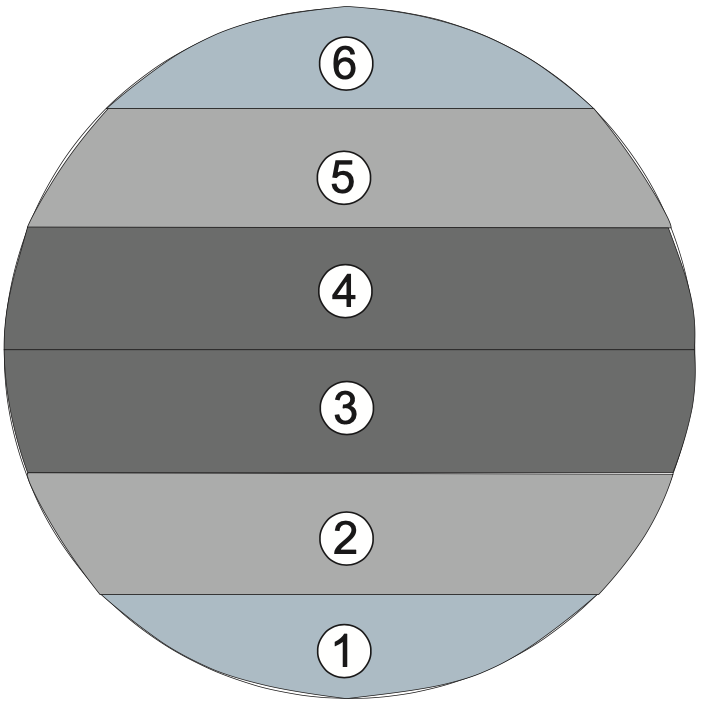
\includegraphics[scale=0.3]{zones.png}
    \caption{Latitude zone intervals.}
    \label{fig:zones}
\end{figure}
\FloatBarrier

Within each zone, temperature evolves through radiative heat fluxes entering the
earth through solar radiation, heat fluxes leaving the earth as long-wave
radiation and the exchange of heat between zones. These effects are quantified
through
\begin{equation} \label{eqn:budyko}
    \frac{dT_k}{dt} = \frac{1}{\mean{\rho_kc_k[Z_k]}}
    \{
      \gamma_k(1-\alpha_k^{sky})(1-\Bar{\alpha}_k)S_0-\tau\sigma_BT_k^{4}
    \} +
    \frac{L_{ki}k_{ki}}{{A_k}\mean{\rho_kc_k[Z_k]}}(T_{k}-T_{i})
\end{equation}
where $k = 1,\dots,6$ represents each latitudinal zone and $T_k$ is the zonal
temperature. The remaining constants are defined in tables \ref{tab:zoneparams}
and \ref{tab:globalparams} of section \ref{sec:Parameters}.

\subsection{Volcanic Eruptions} \label{sec:Volcanos}
Volcanism is an important natural cause of climate change across a range of
timescales \parencite{robock}. For our investigation, we consider the
short-term cooling effects of volcanism that occur on a $10-100$ year time frame.
These cooling effects are introduced in our model by applying an occlusion factor,
$\phi(t)$, to each zone in the model. The
occlusion factor represents the presence of volcanic aerosols suspended in the
atmosphere that block direct shortwave solar radiation.
The introduction of $\phi_k(t)$
transforms equation \ref{eqn:budyko} to
\begin{equation} \label{eqn:occlusion}
\frac{dT_k}{dt} = \frac{1}{\mean{\rho_kc_k[Z_k]}}
\{
    \phi_k(t)\gamma_k(1-\alpha_k^{sky})(1-\Bar{\alpha}_k)S_0-\tau\sigma_BT_k^{4}
\} +
\frac{L_{ki}k_{ki}}{{A_k}\mean{\rho_kc_k[Z_k]}}(T_{k}-T_{i})
\end{equation}
A value of $\phi(t) = 1$ represents no volcanic aerosol occlusion. A value
of $\phi(t) = 0.7$, for example, represents a $30\%$ reduction in total
incoming solar radiation.

\subsubsection{Direct Radiation Occlusion} \label{sec:Occlusion}
Based on observations of the reduction of solar radiation after the
1982 El Chichón eruption and the 1991 Pinatubo eruption \parencite{robock},
an empirical curve for $\phi(t)$ was fit to the data, as shown
in figure \ref{fig:occlusion}. We found that a function with the form
$\phi(t) = 1 - ct^{-2}$, where $c=5.36$ yr$^2$ is an empirical constant found through
nonlinear regression, gave a reasonable representation of the data.
Moreover, this function has the property that $\phi(t) \to 1$ as $t \to \infty$,
which models the decaying effects of aerosol occlusion over time.

\begin{figure}[H]
    \centering
    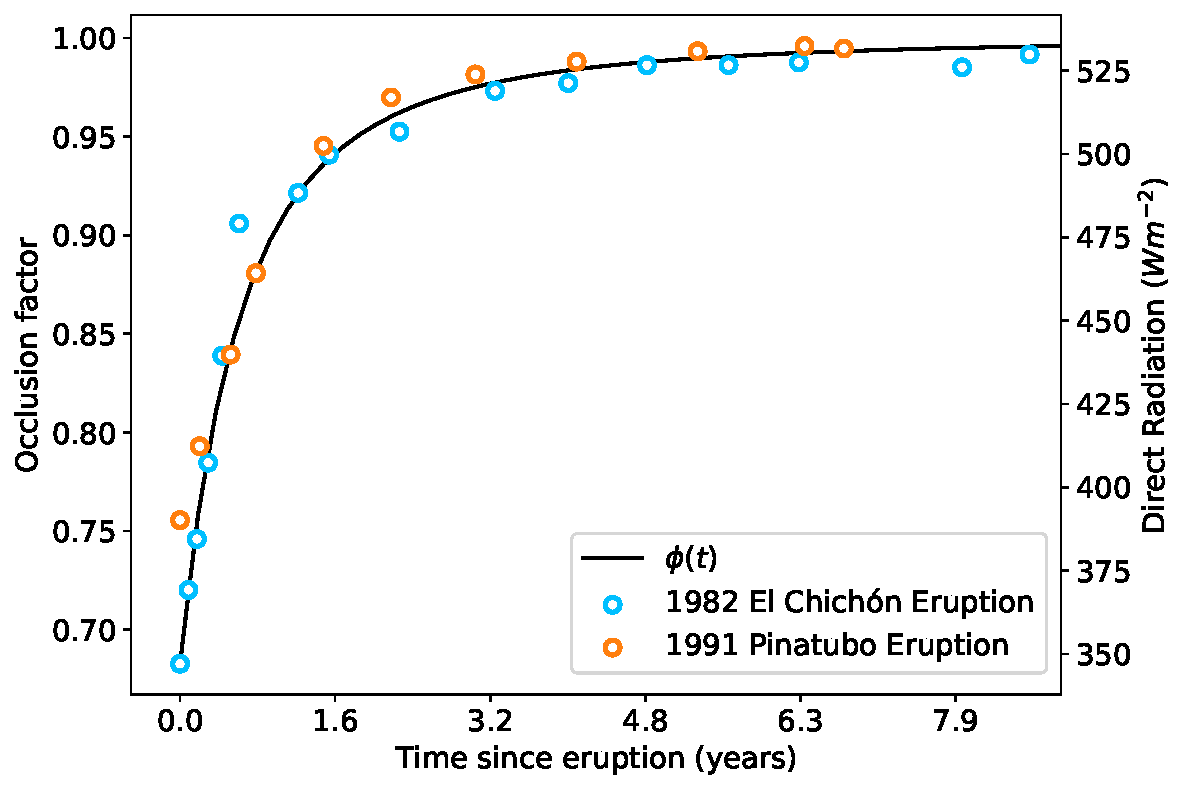
\includegraphics[scale=0.6]{occlusion.pdf}
    \caption{
        Plot of $\phi(t)$; occlusion factor. An occlusion factor of 0.7
        represents a $30\%$ reduction in total incoming solar radiation.
    }
    \label{fig:occlusion}
\end{figure}
\FloatBarrier

\subsubsection{Spatial Distribution of Aerosols} \label{sec:Spatial_Occlusion}
The effects of a volcanic eruption are not local to a single zone. Suspended
aerosols are dispersed throughout the atmosphere and can travel large distances
across the Earth. To model the spatial effects of aerosol dispersion following
an eruption, a time lag is introduced to the zonal occlusion functions,
$\phi_k(t)$, that varies based on the distance zone $k$ is from the eruption
zone. An example is shown in figure \ref{fig:occlusion_space}, where an eruption
occurs at $t=0$ in zone $1$. For the first $3$ months following the eruption,
only zone 1 has the occluding effects of volcanic aerosols. After $3$ months,
the aerosols have traveled to the adjacent zone 2, where $\phi_2(t)$ begins
to follow the decaying occlusion function defined in section \ref{sec:Occlusion}.
This process continues until the entire earth is affected by the volcanic
aerosols after approximately 9 months. The specific lag times considered in the
model were estimated from the data presented in \cite{robock}.

\begin{figure}[H]
    \centering
    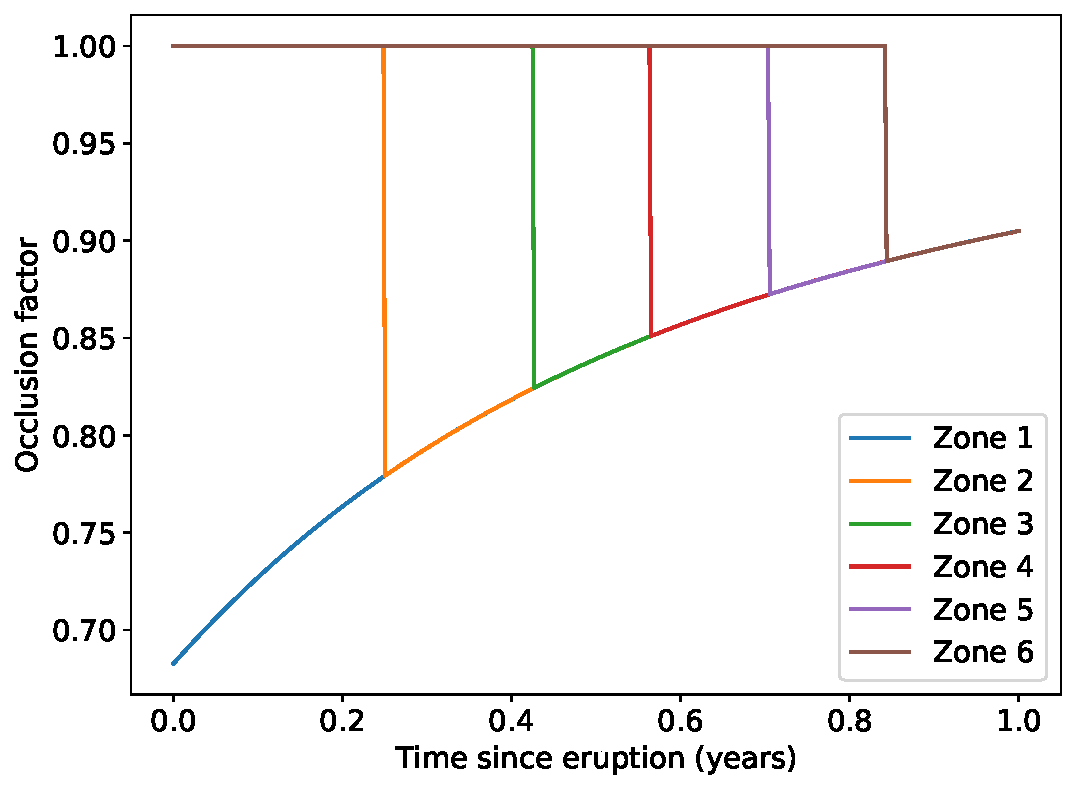
\includegraphics[scale=0.6]{occlusion_space.pdf}
    \caption{
        The spatial effect of eruptions. A distance-dependent time lag is
        present for zones adjacent to the eruption.
    }
    \label{fig:occlusion_space}
\end{figure}
\FloatBarrier

\subsubsection{Stochastic Eruption Frequency} \label{sec:Stochastic}
Sections \ref{sec:Occlusion} and \ref{sec:Spatial_Occlusion} define our model's
response to a single eruption. To investigate the intensity of
volcanism on the Earth's climate, we allow for a series of eruptions to occur
over time. Volcanic eruptions in each zone are modeled as a Poisson
process, where each zone is prescribed an eruption frequency intensity,
$\lambda_k$, that reflects the average repose time between eruptions in the zone.
For an eruption intensity $\lambda_k$, the probability of a repose time, $t_{R}$,
between eruptions follows an exponential distribution
\begin{equation} \label{eq:exponential}
P(t_{R}) = \lambda_k e^{-\lambda_k t_{R}}
\end{equation}
For this investigation, we assume eruptions occur independently in each zone. \\

The intensity of volcanic activity on Earth can be adjusted by raising or
lowering each zone's $\lambda_k$. A smaller $\lambda_k$ represents shorter repose
times and higher volcanic activity. Combining equation \ref{eq:exponential} with
the occlusion function defined in sections \ref{sec:Occlusion} and
\ref{sec:Spatial_Occlusion} gives a simple stochastic model for volcanism on
Earth that includes the time-decaying effects of aerosol occlusion, the spatial
dispersion of aerosols and temporal volcanic intensity.

\subsection{Ice-Albedo Feedback} \label{sec:Ice}
The volcanism defined in section \ref{sec:Volcanos} provides a mechanism to
cool the Earth by occluding direct solar radiation with suspended volcanic
aerosols. One interesting way to study the implications of this cooling is by
considering the ice-albedo feedback \cite{budyko_albedo}. The idea of the
ice-albedo feedback is that if the temperature of the Earth is cold enough,
ice will grow and cover a larger proportion of the Earth's surface. This
will result in a higher surface albedo, reflecting the incoming solar radiation.
The higher albedo will further contribute to decreasing the temperature of
the Earth, leading to a positive feedback. This runaway cooling has the potential
to completely cover the Earth in ice, leading to a ``Snowball Earth'' scenario. \\

We model the ice-albedo feedback by defining a temperature dependent albedo
as follows
\begin{equation} \label{eqn:albedoparam}
    \alpha_k(T_k) =
      \begin{cases}
      \alpha_{k0} & T_k \geq T_0 \\
      \alpha_{k0} + (\alpha_i-\alpha_k)\frac{(T_k-T_0)^2}{(T_i-T_0)^2}
      & T_i < T_k < T_0 \\
      \alpha_i & T_k \leq T_i
      \end{cases}
\end{equation}
where $\alpha_k$ is the albedo in zone $k$, $T_k$ is the temperature in
zone $k$, $T_0 = 280$ K is the threshold temperature where we allow the
growth of ice to increase the albedo, $T_i = 250$ K is the temperature
where the zone is completely covered in ice, $\alpha_{k0}$ is the baseline
zonal albedo given in table \ref{tab:zoneparams} and $\alpha_i = 0.6$ is the
albedo of ice. Figure \ref{fig:albedotemp} shows the nonlinear albedo function
for each zone.

\begin{figure}[H]
    \centering
    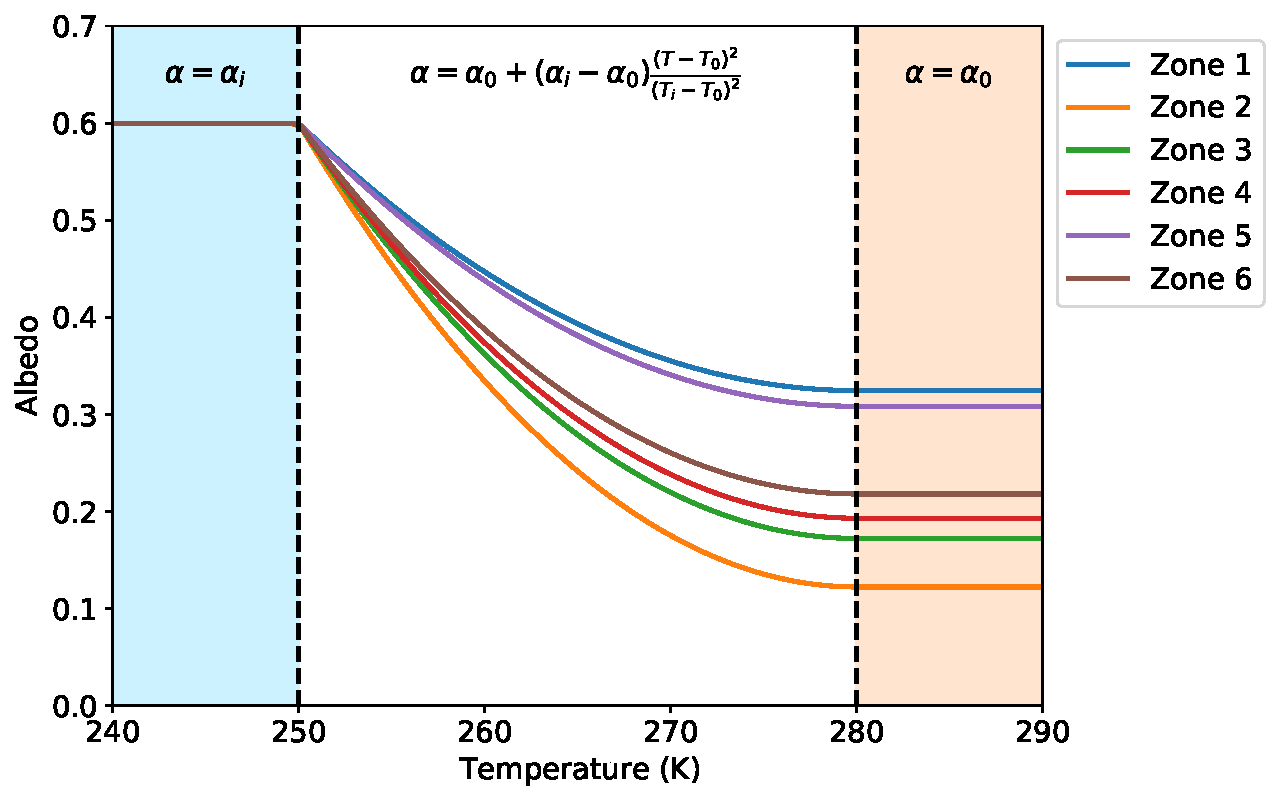
\includegraphics[scale=0.6]{albedo.pdf}
    \caption{
        Albedo parameterization as a function of temperature in each zone.
        The blue shaded region indicates the temperature range where a zone
        is covered with ice. The orange shaded region indicates the temperature
        range where there is no change in ice as temperature varies.
    }
    \label{fig:albedotemp}
\end{figure}
\FloatBarrier

% Figure results
\section{Results}
\label{section:results}
In this section, we will report on data obtained via our three forms of volcanic
perturbations and describe the behaviours of these perturbations within the
context of the data itself.

\subsection{Steady-State Climate Model: No Volcanism}
By passing initial condition temperatures calculated through our model with
suppressed inter-zonal transfer (See Table \ref{tab:teq}) to our
steady-state model where inter-zonal transfer is allowed, we solve for the
equilibrium temperatures by integrating forward in time
(Figure \ref{fig:steadystate}).

\begin{table}
    \centering
    \begin{tabular}{ c | c | c }
        \hline
        \thead{Zone} &
        \thead{Interzonal Transfer Supressed \\ Equilibrium Temperature [K]} &
        \thead{Interzonal Transfer Allowed \\ Equilibrium Temperature [K]} \\
        \hline
        1 & 217.23 & 274.12 \\
        2 & 279.74 & 279.34 \\
        3 & 296.45 & 282.26 \\
        4 & 294.56 & 280.88 \\
        5 & 263.56 & 279.71 \\
        6 & 225.33 & 274.93 \\
        \hline
    \end{tabular}
    \caption{
        Equilibrium Temperature distributions for a climate model with no
        volcanism
    }
    \label{tab:teq}
\end{table}

\begin{figure}[H]
    \centering
    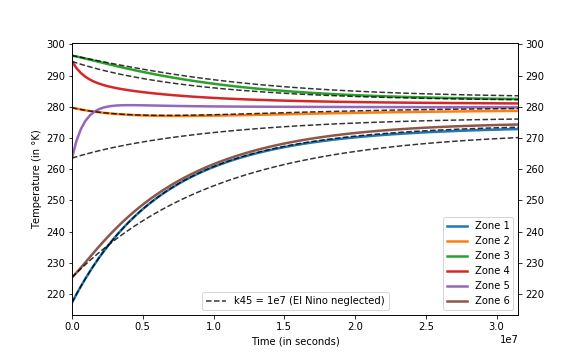
\includegraphics[scale=0.5]{Question2.png}
    \caption{
        Equilibrium solution for 6-zoned Earth climate model. Zone 1 marks the
        southernmost band at $60-90^{\circ}$S while zone 6 represents the
        northernmost band at $60-90^{\circ}$N. Zones 2-5 are bands covering
        $30^{\circ}$ intervals between zones 1 and 6
        (See Figure \ref{fig:zones}).
    }
    \label{fig:steadystate}
\end{figure}
\FloatBarrier

There are a few key observations to note. The first is that a larger transfer
coefficient (\ref{tab:boundaryparams}), representing the northern Gulf Stream
between zones 4 and 5, produces a large initial temperature gradient in these
zones relative to the others (solid colour lines in Figure
\ref{fig:steadystate}). The second is that the highest temperature zones at
equilibrium are 3 and 4, and the lowest temperature zones at equilibrium are 6
and 1. All zones approach an equilibrium temperature between $274.1^{\circ}$K
and $282.3^{\circ}$K after a model year (Table \ref{tab:teq}). By reducing the
inter-zonal transfer coefficient between zones 4 and 5
(dashed lines in Figure \ref{fig:steadystate}), we can alter the characteristics
of a few zones dramatically. The most obvious of which are zones 4, 5, and,
perhaps surprisingly, zone 6. These alterations include a reduction in the
initial rate of change in temperature and will be analyzed further in Section
\ref{section:steadystate}.

\subsection{Climate Model Following Single Volcanic Eruption}
Figure \ref{fig:oneerupt} shows the effect of a single eruption on zonal 
temperatures initially at steady-state. The eruption occurs in zone 4 after
1 year, as indicated by the vertical dashed line.
Zone 4 is immediately affected by the solar occlusion and shows a decrease
in temperature. A time lag between the zonal temperature responses is clearly
visible with zones at a greater distance from zone 4 showing a larger time lag.
The recovery of each zone to its equilibrium temperature occurs over approximately
15 years after the eruption. The equilibrium temperature values are the same
post-eruption as they are pre-eruption.

\begin{figure}[H]
    \centering
    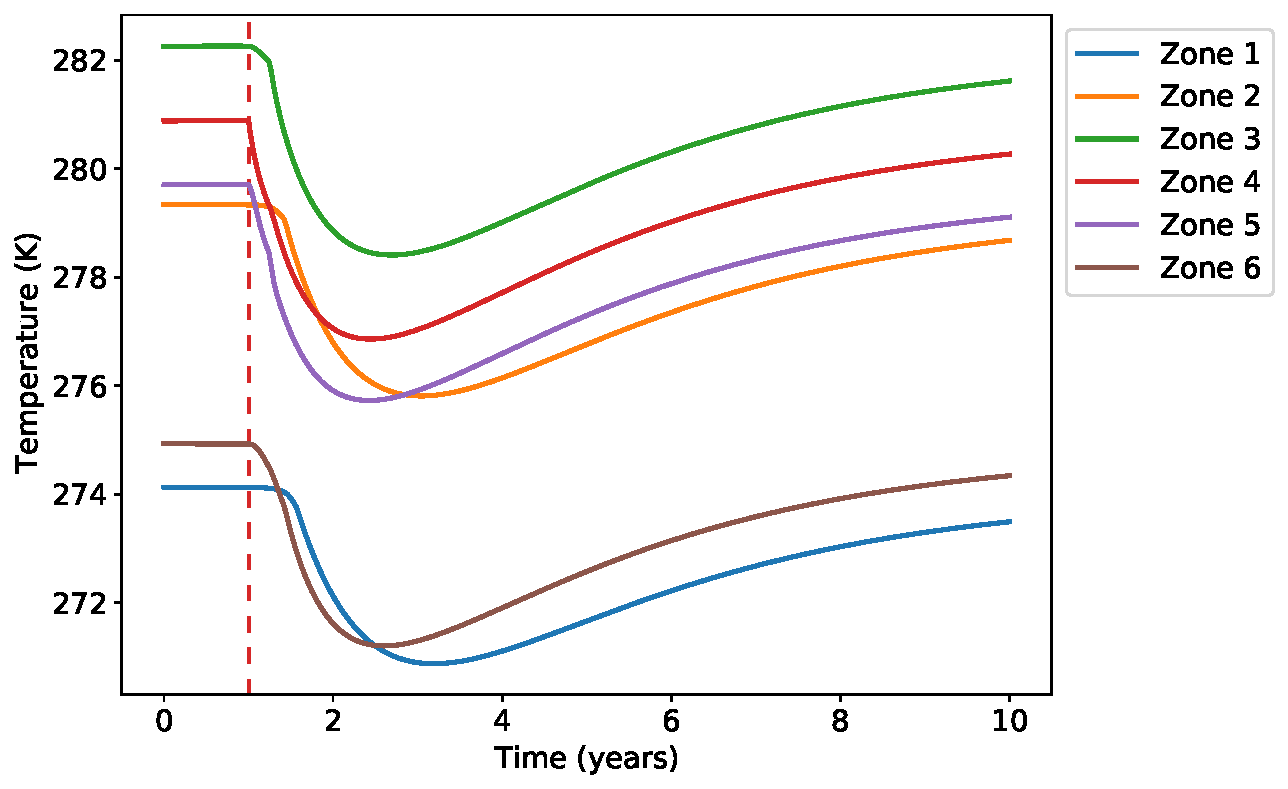
\includegraphics[scale=0.6]{one_eruption.pdf}
    \caption{
        Reduction in solar forcing post eruption results in temperature drop.
    }
    \label{fig:oneerupt}
\end{figure}
\FloatBarrier

\subsection{Stochastic Volcanic Eruptions}
Figure \ref{fig:stocherupt} shows a model result that includes multiple
eruptions following the Poisson process defined in section \ref{sec:Stochastic}.
Vertical dashed lines represent an eruption with a coloured by the zone the eruption
occurred. The eruption intensity parameters used are given in table
\ref{tab:lambda_stochastic}
\begin{table}
    \centering
    \begin{tabular}{ c | c }
      \hline
      \thead{Zone} & 
      \thead{$\lambda_k [\text{yr}^{-1}]$} \\
      \hline
      1 & 100 \\
      2 & 50 \\
      3 & 20 \\
      4 & 20 \\ 
      5 & 50 \\
      6 & 100 \\
    \hline
    \end{tabular}
    \caption{Volcanic intensity rate parameters}
    \label{tab:lambda_stochastic}
\end{table}
\begin{figure}[H]
    \centering
    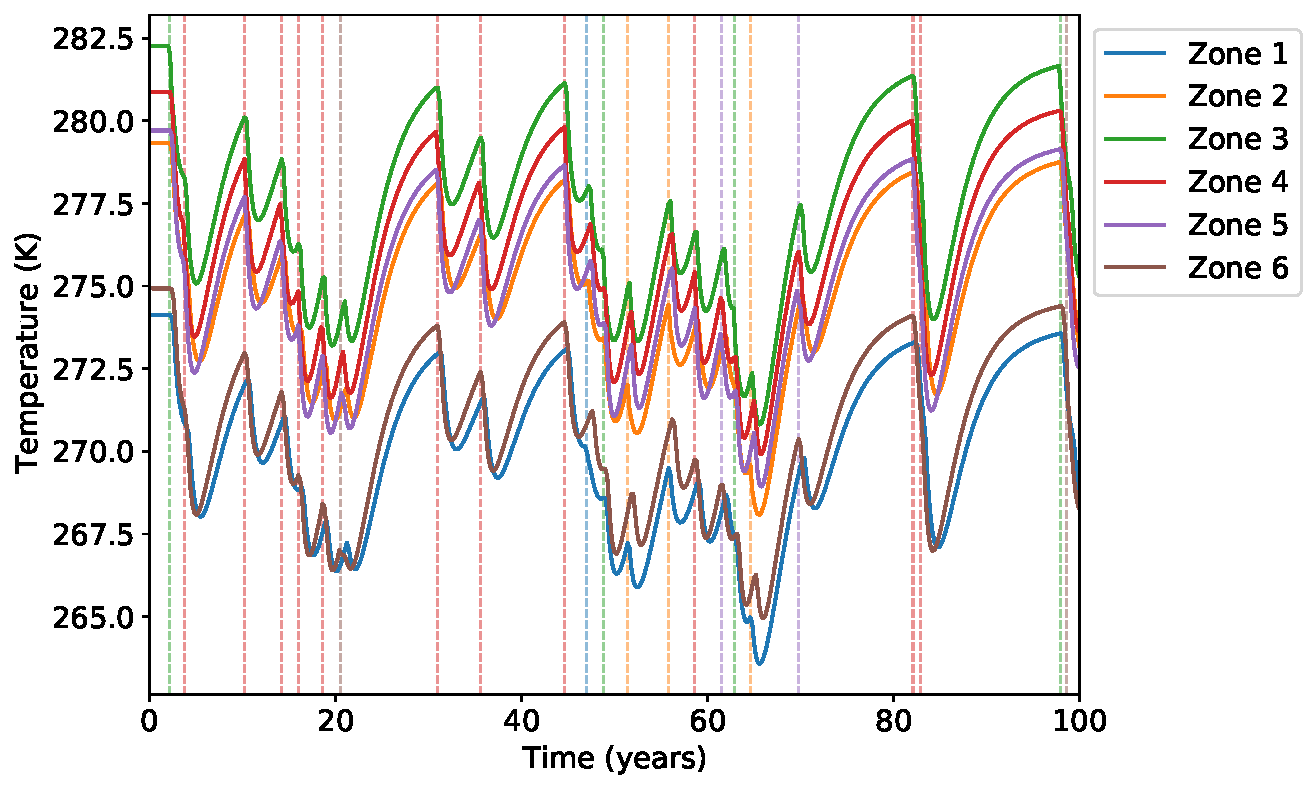
\includegraphics[scale=0.6]{stochastic_eruptions.pdf}
    \caption{
        Stochastic eruption distribution following Poisson distribution.
        Vertical dotted lines are colored based on the zone the eruption
        occurred in, and their placement is the point in time at which the
        eruption is initiated.
    }
    \label{fig:stocherupt}
\end{figure}
\FloatBarrier

The model was run for 100 years to show multiple cycles of temperature
drops and recoveries. From Figure
\ref{fig:stocherupt}, we see that following each eruption is a decline in zonal
temperatures, and sufficiently close eruptions, in time, compound that effect.
The distribution lag associated with aerosol spreading is still represented
numerically, though a lag of a few months is difficult to discern visually on
this extended time scale. 

\subsection{The Ice-Albedo Effect} \label{sec:ice_albedo_results}
Figure \ref{fig:albedo_equil} shows the result of the temperature dependent albedo
from in equation \ref{eqn:albedoparam} coupled with our climate model in
equation \ref{eqn:budyko}. The temperature ranges for the nonlinear albedo model
are coloured similar to figure \ref{fig:albedotemp}. We recognize three temperature equilibria,
two of which are stable and one that is unstable. The equilibrium temperature
distributions are shown in table \ref{tab:eqstates}.

\begin{table}
    \begin{tabular}{ c | c | c | c }
      \hline
      \thead{Zone} & 
      \thead{Warm Earth \\ Equilibrium Temperature [K]} &
      \thead{Unstable \\ Equilibrium Temperature [K]} &
      \thead{Snowball Earth \\ Equilibrium Temperature [K]} \\
      \hline
      1 & 274.02 & 251.08 & 231.91 \\
      2 & 279.27 & 255.03 & 234.30 \\
      3 & 282.21 & 258.31 & 236.23 \\
      4 & 280.83 & 257.78 & 236.13 \\ 
      5 & 279.66 & 256.98 & 235.70 \\
      6 & 274.83 & 253.11 & 233.20 \\
        \hline
    \end{tabular}
    \caption{Ice-albedo effect equilibrium temperature distributions}
    \label{tab:eqstates}
\end{table}

\begin{figure}[H]
    \centering
    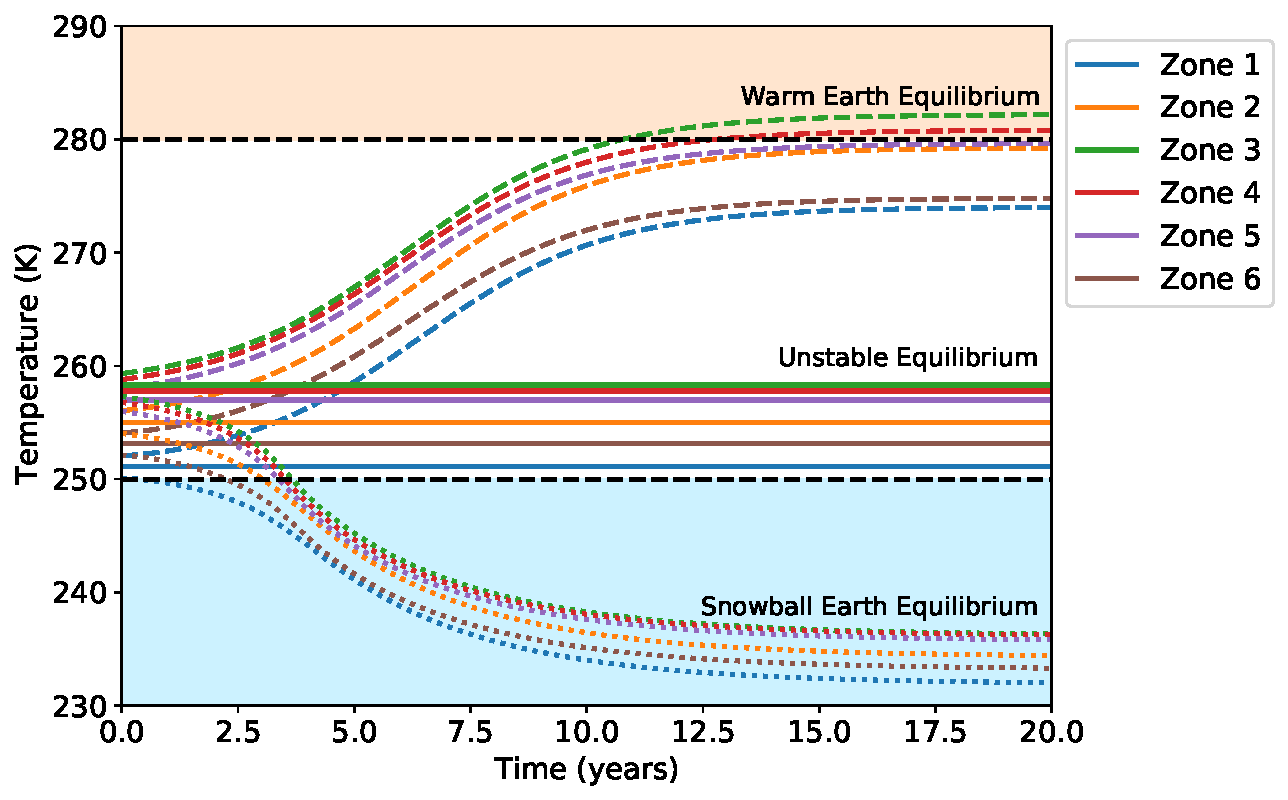
\includegraphics[scale=0.6]{albedo_equilibria_1plot.pdf}
    \caption{
        Integrating through climate model incorporating both stochastic volcanic
        eruptions and ice-albedo feedback parameterization.
    }
    \label{fig:albedo_equil}
\end{figure}
\FloatBarrier

A model started with an initial temperature distribution at the unstable equilibrium
(solid lines in figure \ref{fig:albedo_equil}) remains at the unstable equilibrium. \\

A model started with an initial temperature distribution perturbed slightly above
the unstable equilibrium (dashed lines in figure \ref{fig:albedo_equil}) asymptotically
approaches the ``warm Earth'' equilibrium given in table \ref{tab:eqstates}. \\

A model started with an initial temperature distribution perturbed slightly below
the unstable equilibrium (dotted lines in figure \ref{fig:albedo_equil}) asymptotically
approaches the ``snowball Earth'' equilibrium given in table \ref{tab:eqstates}.
The temperature difference between high-latitudinal and mid-latitudinal zones is much
smaller for the snowball Earth equilibrium compared to the warm Earth equilibrium.

\subsection{Fire and Ice: Stochastic Volcanism and the Ice-Albedo Feedback}
Figure \ref{fig:fireandice} shows the results of two models that combine
volcanism defined in section \ref{sec:Volcanos} with the ice-albedo feedback
defined in section \ref{sec:Ice}. The temperature ranges for the nonlinear albedo model
are coloured similar to figure \ref{fig:albedotemp}. The ``Stable Eruption Frequency'' and
``Unstable Eruption Frequency'' models were forced with the eruption intensity
rate parameters shown in table \ref{tab:lambda_stochastic_ice}.

\begin{table}
    \centering
    \begin{tabular}{ c | c | c}
      \hline
      \thead{Zone} & 
      \thead{Stable Eruption Frequency \\ $\lambda_k [\text{yr}^{-1}]$} &
      \thead{Unstable Eruption Frequency \\ $\lambda_k [\text{yr}^{-1}]$} \\
      \hline
      1 & 150 & 100 \\
      2 & 75 & 50 \\
      3 & 50 & 20 \\
      4 & 50 & 20 \\ 
      5 & 75 & 50 \\
      6 & 150 & 100 \\
    \hline
    \end{tabular}
    \caption{
        Volcanic intensity rate parameters for the volcanism with ice-albedo
        feedback models
    }
    \label{tab:lambda_stochastic_ice}
\end{table}

\begin{figure}[H]
    \centering
    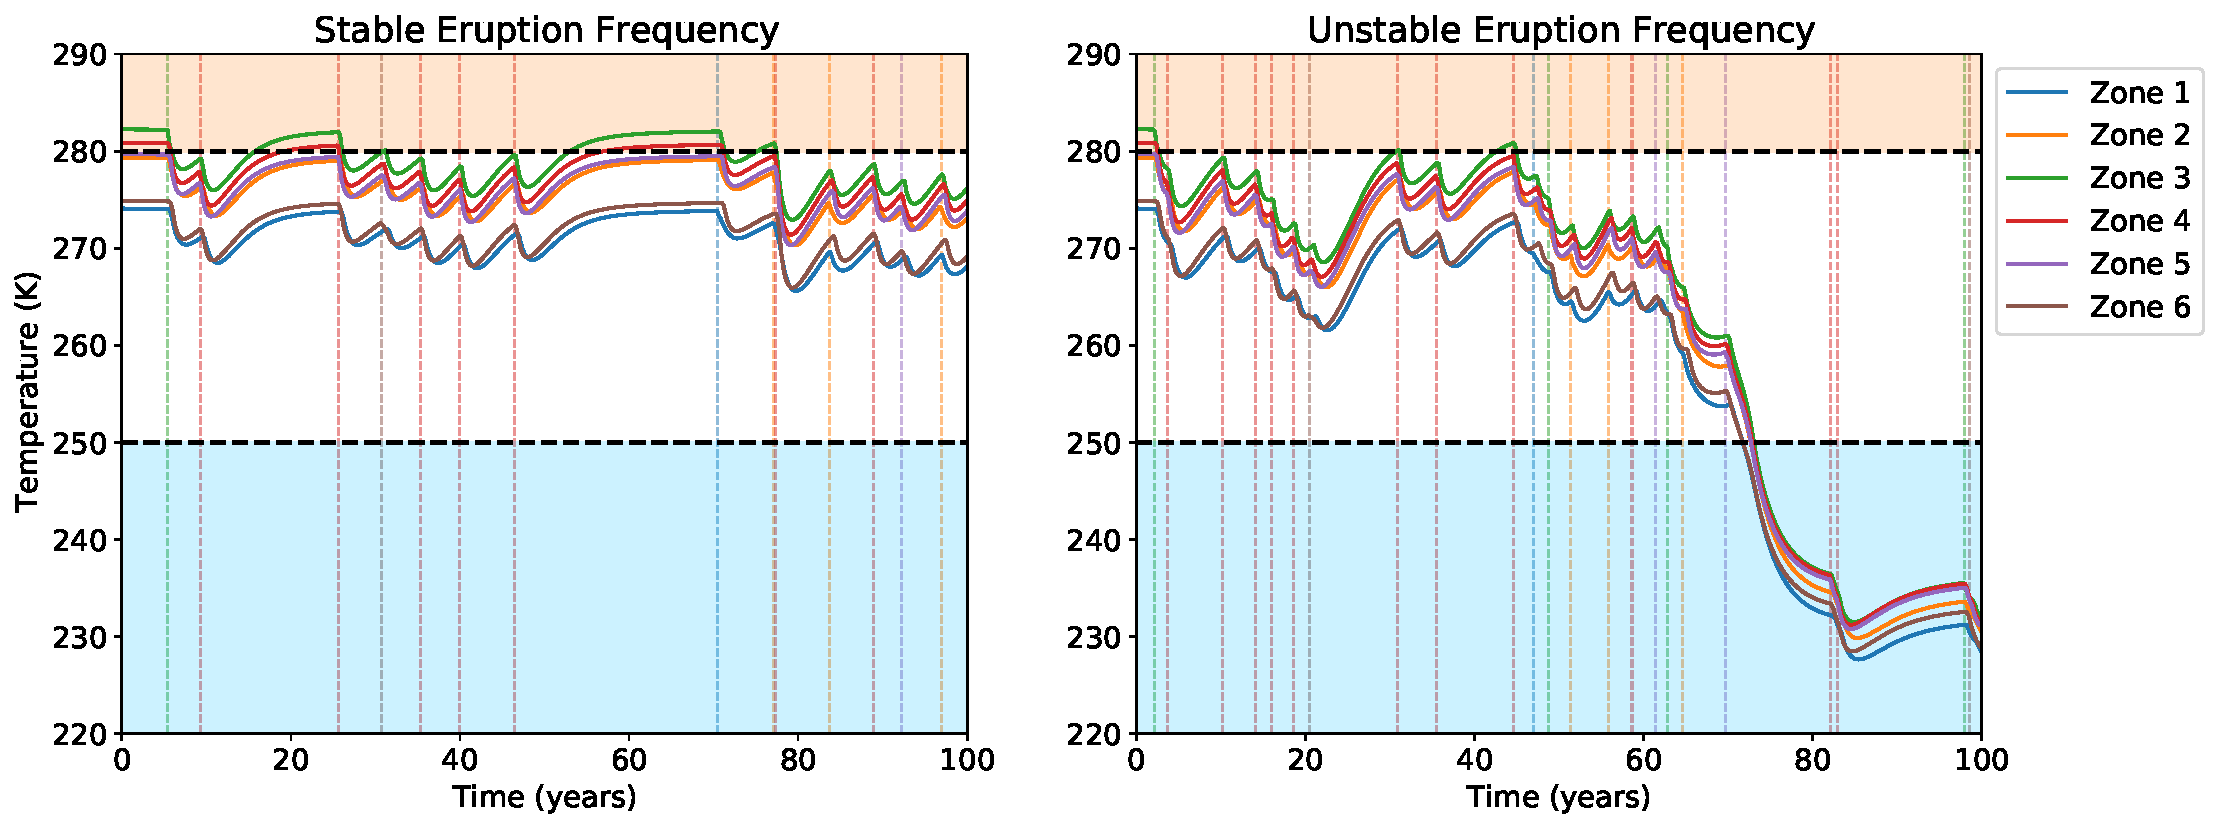
\includegraphics[width=\linewidth]{eruptions_albedo.pdf}
    \caption{
        Model results for volcanism combined with the ice-albedo feedback.
    }
    \label{fig:fireandice}
\end{figure}
\FloatBarrier

The stable eruption frequency model oscillates around the warm Earth equilibrium
shown in section \ref{sec:ice_albedo_results}. The unstable eruption frequency
oscillates around the warm Earth equilibrium for approximately
$70$ years before it quickly drops to oscillate around the snowball
Earth equilibrium.

\section{Discussion}
Here we will discuss the possible processes behind the numerical behavior of our
Figures in Section \ref{section:results} in order to elucidate the connection
between our mathematical and computational results with their underlying
physics.

\subsection{Steady-State Climate Model: No Volcanism}
\label{section:steadystate}
Zones 4 and 5 experience a large initial temperature gradient due to a heat
transfer coefficient indicative of Gulf Stream circulation processes that is
larger than the transfer coefficients between other zones
(Figure \ref{fig:steadystate}). This causes zones 4 and 5 to approach their
equilibrium values more quickly. For example, zone 5 reaches its approximate
equilibrium temperature within the first two months of the model year because
the efficiency of heat transfer between these zones is greater than between
others. \\

Zones 3 and 4 are the warmest zones due to their proximity to Earth's equator.
Both lie within $30^{\circ}$N/S of the equator, and hence have the largest
effective surface area, coupled with a low albedo due to a high land and sea
fraction versus ice fraction (See Table \ref{tab:zoneparams}). This increases
these zones' retention of incoming solar radiative heating by reducing the
amount lost to space as out-going, long-wave radiation (OLR). Zone 3 may be
hotter than zone 4 due to smaller transfer coefficients between its adjacent
zones than compared with zone 4, where heat transfer occurs rapidly due to
influence from the Gulf Stream across the boundary of zone 4 and 5. \\

Conversely, zones 1 and 6 are the coldest zones at equilibrium due to their
placement at Earth's high latitudes ($>60^{\circ}$N/S). This reduces their
effective surface area such that less total solar insolation occurs, alongside
a higher albedo due to a dominating ice fraction. This causes the OLR to be
larger relative to incoming radiative heating than in the case of the other
zones. Hence, temperature at equilibrium in zones 1 and 6 is lower. Zone 1 may
be colder than zone 6 due to a higher albedo associated with a marginally larger
ice fraction that increases OLR even relative to zone 6. \\

Comparing the solid and dashed lines in Figure \ref{fig:steadystate}, there is a
general trend of reduced rate of change in temperature for several northern 
latitudinal zones. Zones 4 and 5 experience the greatest deviation from the
original approach to equilibrium as this change is at their boundary of
separation and directly reduces the amount of heat exchange between them.
Zone 6 also experiences a reduction in the rate of approach to equilibrium due
to its nonlinear relation with zone 5. As we can see, these effects are
compounded in zones closest to zones 4 and 5, such that at sufficient
separation, approaches to equilibrium are not noticeably affected. This is
evident in zones 2 and 1, and suggests they have little dependence on
temperature characteristics within the northern zones. 

\subsection{Volcanic Eruptions}
One of the aims of our study was to investigate the short-term impact of
volcanism on Earth's climate. The occlusion factor introduced in section
\ref{sec:Occlusion} ultimately acts to cool the climate by blocking direct
solar radiation from reaching the Earth's surface.\\

An interesting result is the difference in time scales for the occluding effect
of an eruption and the subsequent recovery time of the climate. Figure
\ref{fig:occlusion} shows that suspended aerosols block less than 5\% of
direct solar radiation 2 years after an eruption. On the other hand, figure
\ref{fig:oneerupt} shows that it takes over a decade before the climate recovers
to within 5\% of its equilibrium temperature. This demonstrates that the climate
feels the effects of volcanic aerosol occlusion even after the aerosols have
dissipated and no longer block solar radiation. \\

The longer recovery time increases the susceptivity of the climate to compounding
temperature drops from multiple eruptions, as see in figure \ref{fig:stocherupt}.
Temperatures are forced to values over 10 degrees below their equilibrium values
during intense volcanic episodes. As we will see, these high intensity volcanic
episodes can be a trigger that drives to Earth away from its initial equilibrium
into a snowball Earth state.

\subsection{The Ice-Albedo Effect}
The nonlinear albedo dependence on temperature defined in equation
\ref{eqn:albedoparam} ultimately gives rise to three equilibrium
conditions, as illustrated in figure \ref{fig:albedo_equil}. The ``warm Earth''
equilibrium represents conditions where the ice-albedo feedback has a small
effect on the Earth's global energy balance. A small decrease in temperature
near this equilibrium is compensated by an increase in heat flow from adjacent
zones as well as a net positive flux of radiative energy from the sun which acts to
increase the temperature. Even when
temperatures fall in the variable albedo temperature range
(i.e. $250 \text{K} < T < 280 \text{K}$), no ice-albedo runaway is observed.
There is a slight decrease in equilibrium temperatures
for the warm Earth equilibrium when compared to the equilibrium for the model with
no ice-albedo feedback (\ref{tab:teq} and \ref{tab:eqstates}) due to some of
the equilibrium temperatures falling in the variable albedo range.


\subsection{Fire and Ice: Stochastic Volcanism and the Ice-Albedo Feedback}
\label{sec:snowballearth}

\section{Conclusion}
We saw that:
In that case, under what conditions could Earth recover form the snowball solution?
This model only investigates the effects of SO2 on the energy balance, not considering
the influence of CO2. CO2 is a greenhouse gas, meaning that it efficiently absorbs the
incoming solar radiation Volcanic eruptions 
\subsection{Future Work}

\section{Ancillary Information}
\subsection{Author Contributions}

\begin{table}[H]
    \centering
    \begin{tabular}{rrr}
    Section & Subsection & Contributors \\
    \hline
    Graphic & Box-Model & M  \\
    Code & Steady-State Climate & P and E \\
    Code & Perturbation: Single Volcanic Eruption & P, E, and M \\
    Code & Snowball Earth & P, E, and M \\
    Introduction &  & M \\
    Results & Steady-State Climate & n/a \\
    Results & Perturbation: Single Volcanic Eruption & n/a \\
    Results & Snowball Earth & n/a\\
    Discussion & Steady-State Climate Model & n/a \\
    Discussion & Perturbation: Single Volcanic Eruption & n/a \\
    Discussion & Snowball Earth & n/a\\
    Conclusion & Future Work & n/a \\
    Conclusion & Summary & n/a \\
    \end{tabular}
    \caption{
        In descending order: names depict relative contribution to
        sections with more than one contributor.
    }
    \label{tab:contributions}
\end{table}

\subsection{Algorithm Development}

\begin{figure}[H]
    \centering
    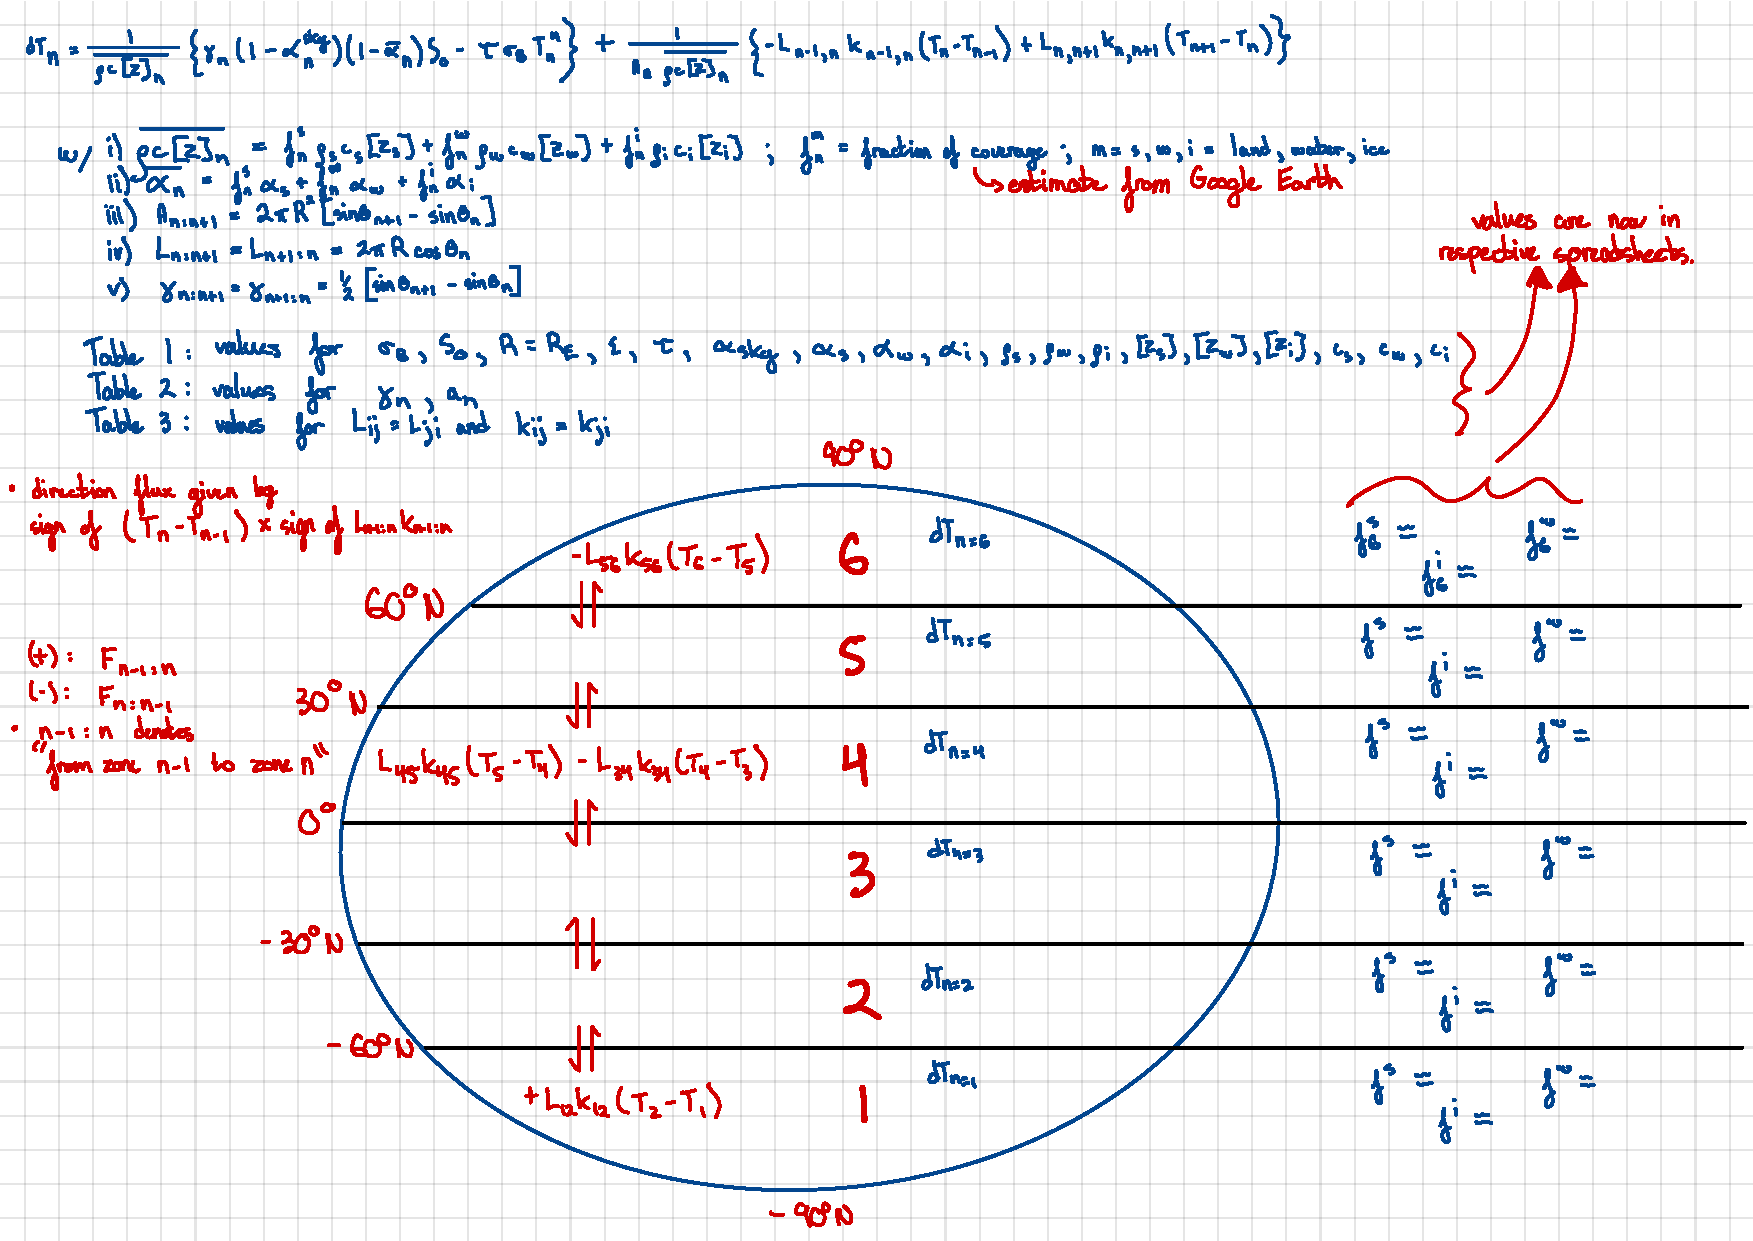
\includegraphics[scale=0.3]{Graphicalg.pdf}
    \caption{
        Sketch depicting zone intervals and necessary parameters for numerical
        solving.
    }
    \label{fig:graphicalg}
\end{figure}
\FloatBarrier

\begin{enumerate}
    \item Identify 6 latitudinal zones. Namely between $0-30^{\circ}NS$,
    $30-60^{\circ}NS$ and $60-90^{\circ}NS$.
    \item Determine parameters associated with each area.
    \item Solve ODE numerically using Paul Matlashewski's
    ClimateModel.py library.  
\end{enumerate}

% \subsection{Python Functions}
% Add your important MATLAB functions here with a brief implementation explanation. This is how to make an \textbf{unordered} list:
% % \begin{itemize}
% %     \item \texttt{y = linspace(x1,x2,n)} returns a row vector of \texttt{n} evenly spaced points between \texttt{x1} and \texttt{x2}. 
% %     \item \texttt{[X,Y] = meshgrid(x,y)} returns 2-D grid coordinates based on the coordinates contained in the vectors \texttt{x} and \texttt{y}. \text{X} is a matrix where each row is a copy of \texttt{x}, and \texttt{Y} is a matrix where each column is a copy of \texttt{y}. The grid represented by the coordinates \texttt{X} and \texttt{Y} has \texttt{length(y)} rows and \texttt{length(x)} columns.  
% % \end{itemize}

% % Python Codes
% \subsection{Python Code}
% Add your Python code here. This section will not be included in your page limit of six pages.
% \begin{listing}[h]
% \inputminted{matlab}{example.m}
% \caption{Example code from external file.}
% \label{listing:examplecode}
% \end{listing}
\subsection{Data}
\subsubsection{Eruption Times Series}
\begin{table}[H]
    \parbox{.45\linewidth}{
    \captionsetup{singlelinecheck = false, justification=justified}
    \caption{Eruption Times Series 1}
    \label{tab:erupt1}
    \csvautobooktabular{eruption_1.csv}
    }
    \hfill
    \parbox{.45\linewidth}{
    \captionsetup{singlelinecheck = false, justification=justified}
    \caption{Eruption Time Series 2}
    \label{tab:erupt2}
    \csvautobooktabular{eruption_2.csv}
    }
\end{table}

\subsubsection{Parameters} \label{sec:Parameters}
\begin{table}[H]
    \parbox{.45\linewidth}{
    \captionsetup{singlelinecheck = false, justification=justified}
    \caption{Zonal Parameters}
    \begin{tabular}{lll}
    \hline
     & Parameter & Value \\
    \hline
    Zone 1 & Geometric Factor & 0.1076 \\
     & Area Fraction & 0.067 \\
     & Land Fraction & 0.0 \\
     & Ocean Fraction & 0.550925926 \\ 
     & Ice Fraction & 0.449074074 \\
    \hline
    Zone 2 & Geometric Factor & 0.2277 \\
     & Area Fraction & 0.183 \\
     & Land Fraction & 0.074074074 \\
     & Ocean Fraction & 0.925925926 \\ 
     & Ice Fraction & 0.0\\
    \hline
    Zone 3 & Geometric Factor & 0.3045 \\
     & Area Fraction & 0.25 \\
     & Land Fraction & 0.240740741 \\
     & Ocean Fraction & 0.759259259 \\ 
     & Ice Fraction & 0.0\\
    \hline
    Zone 4 & Geometric Factor & 0.3045 \\
     & Area Fraction & 0.25 \\
     & Land Fraction & 0.3101851851 \\
     & Ocean Fraction & 0.689814815 \\ 
     & Ice Fraction & 0.0\\
    \hline
    Zone 5 & Geometric Factor & 0.2277 \\
     & Area Fraction & 0.183 \\
     & Land Fraction & 0.694444444 \\
     & Ocean Fraction & 0.305555556 \\ 
     & Ice Fraction & 0.0\\
    \hline
    Zone 6 & Geometric Factor & 0.1076 \\
     & Area Fraction & 0.067 \\
     & Land Fraction & 0.277777778 \\
     & Ocean Fraction & 0.652777778 \\ 
     & Ice Fraction & 0.069444444\\
    \end{tabular}
    \label{tab:zoneparams}
    }
    \hfill
    \parbox{.45\linewidth}{
    \captionsetup{singlelinecheck = false, justification=justified}
    \caption{Global Parameters}
    \begin{tabular}{lll}
    \hline
    Parameter & Value & Units \\
    \hline
    Stefan-Boltzmann Constant & 5.6696e-8 & $Wm^{-2}K^{-4}$ \\
    Solar Constant & 1368 & $Wm^{-2}$ \\
    Earth Radius & 6371e3 & $m$ \\
    Earth Total Emissivity & 1  \\
    Atmospheric Transmissivity & 0.63  \\
    Atmospheric Albedo & 0.2 \\
    Land Albedo & 0.4 \\
    Ocean Albedo & 0.1\\
    Ice Albedo & 0.6 \\
    Land Density & 2500 & $kgm^{-3}$\\
    Ocean Density & 1028 & $kgm^{-3}$\\
    Ice Density & 900 & $kgm^{-3}$\\
    Land Thermal Scale Depth & 1.0 & $m$ \\
    Ocean Thermal Scale Depth & 70.0 & $m$ \\
    Ice Thermal Scale Depth & 1.0 & $m$ \\
    Land Specific Heat Capacity & 790 & $JkgK^{-1}$\\
    Ocean Specific Heat Capacity & 4187 & $JkgK^{-1}$\\
    Ice Specific Heat Capacity & 2060 & $JkgK^{-1}$\\
    \end{tabular}
    \label{tab:globalparams}}
\end{table}
\FloatBarrier

\newpage
\section{References}
\printbibliography

\end{document}
